% generated by build_assets.py from the recorded PDF and caption; do not edit
\begin{figure}[tbp]
\centering
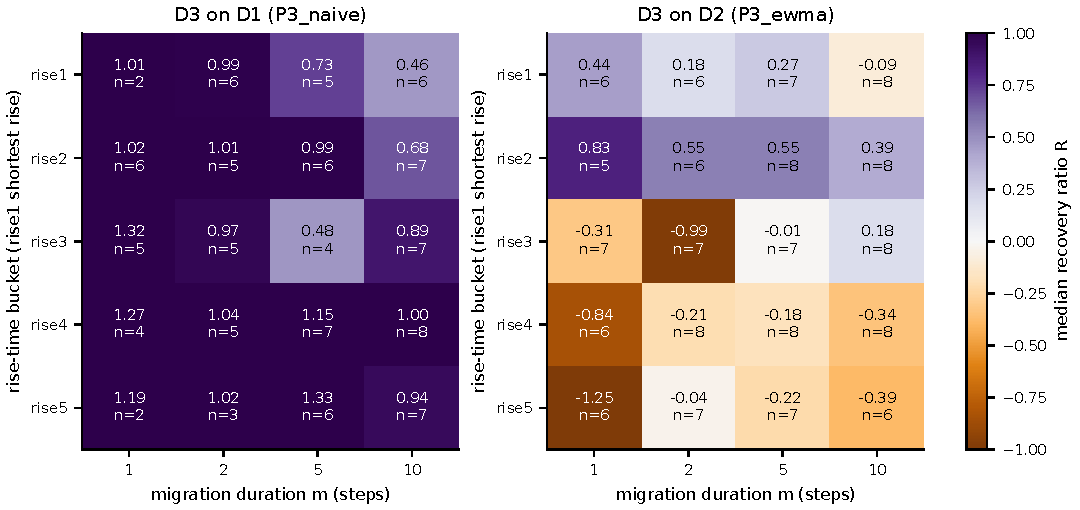
\includegraphics[width=\linewidth]{assets/figures/fa6_regime_q2.pdf}
\caption{FA6a. Measured lag-tax recovery ratio R across migration duration m (x) and flash-crowd rise-time bucket (y), headroom 1.6, injected-event data D3 on D1 and on D2 (forecast policy: P3\_ewma/P3\_naive). Cell text is the median R over events with R defined and the number n of those events (of 8 events per bucket); blank cells have no event with R defined. Colour is clipped to the range -1 to 1, the printed value is not clipped. R is defined only where the lag tax is at least the registered share of the reactive damage. Every cell rests on few events (flag in tables/regime\_map\_q2.csv); intervals are in the table. Datasets are not pooled.}\label{fig:fa6_regime_q2}
\end{figure}
